%\tablesofcontent

\section{Numerical Results}

%% \subsection{Industrial environnment}
%% \begin{frame}{Programmation environnement}

%%   \begin{multicols}{2}
%%     \begin{figure}[H]
%%       \centering
%%       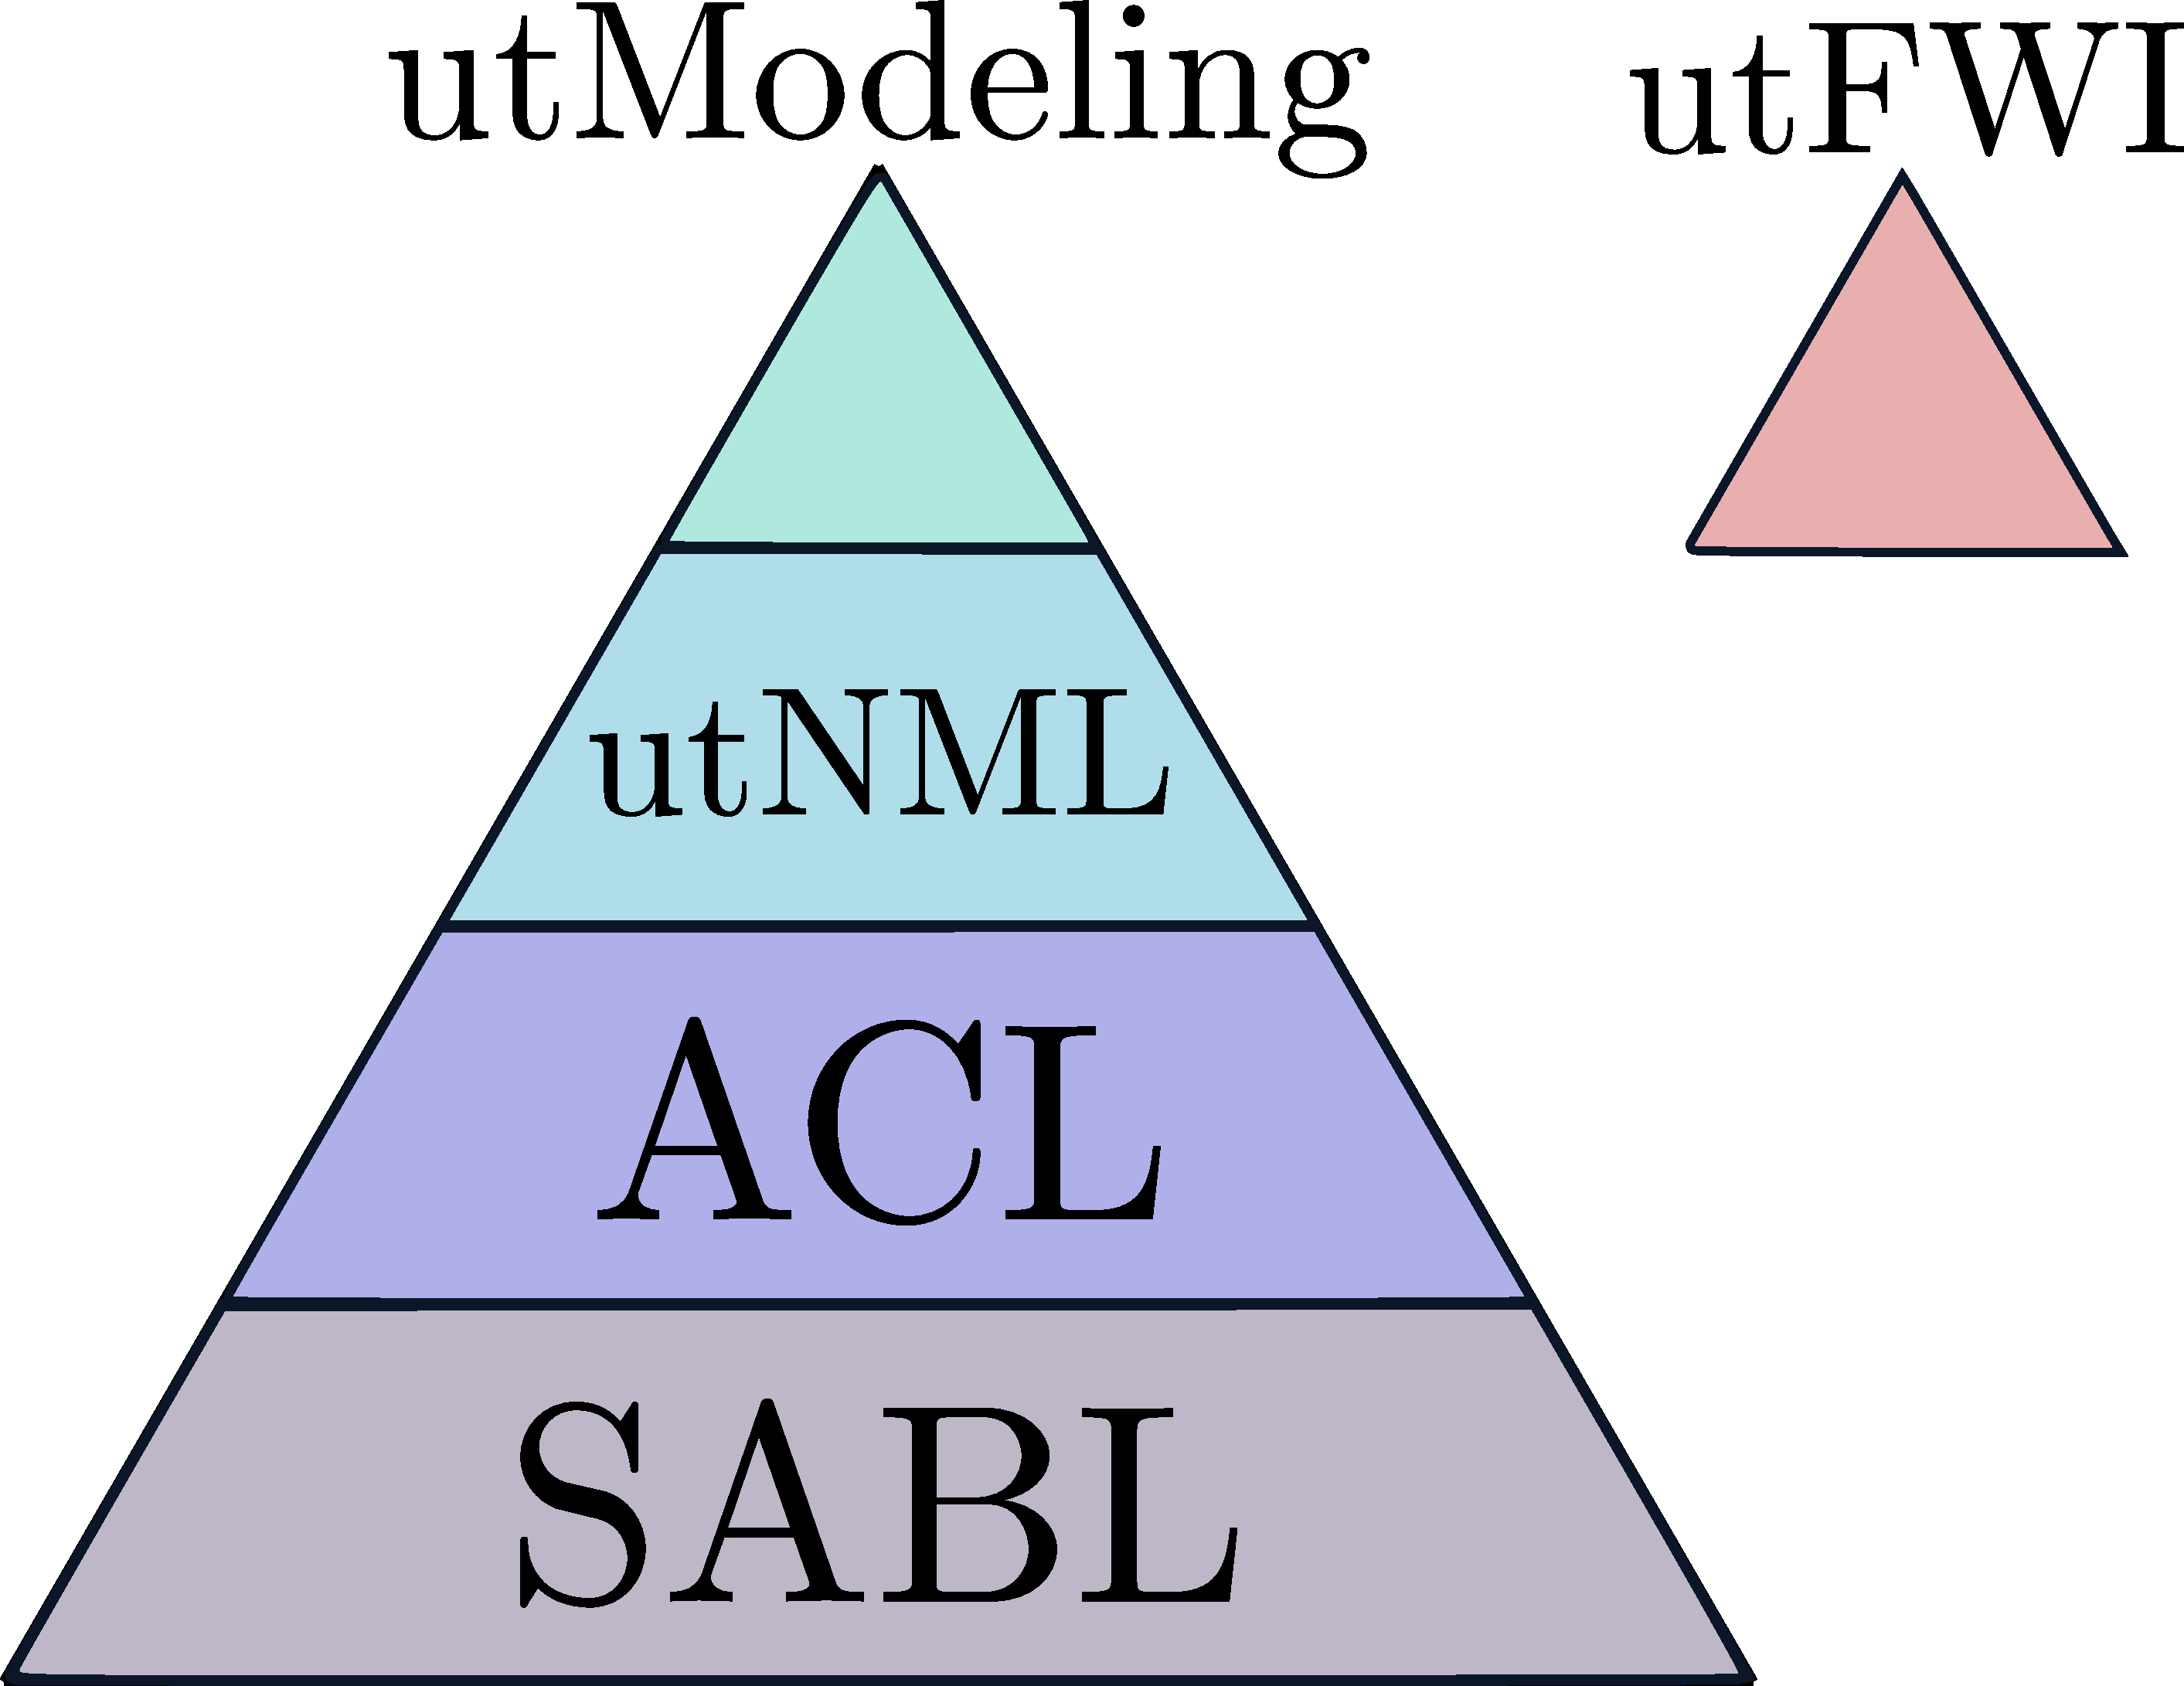
\includegraphics[scale=0.12]{image/carbon.pdf}
%%       \caption*{Illustration of the hierarchical Total's environnement.}
%%       \label{carbon}
%%     \end{figure}

%%     \columnbreak

%%     \begin{itemize}
%%       \small
%%     \item<2-> \textbf{SABL}: Seismic Application Base Library (Seismic acquisition + Parallelism)
%%     \item<3-> \textbf{ACL}: Application Core Library  (Discrete operator + Domain decomposition)
%%     \item<4-> \textbf{utNML}: Unstructured Time-domain Numerical Methods Library (Propagators + Models + Seismic Data management)
%%     \item<5-> \textbf{utModeling}: Unstructured Time-domain Modeling (Main application to perform the modelling)
%%     \end{itemize}
%%   \end{multicols}

%% \end{frame}


\subsection{Parallelism}
\begin{frame}{Parallelism}{Two levels of parallelism}

  \begin{overprint}
    \onslide<2>
  \begin{figure}[H]
    \centering
    
\includegraphics[scale=0.15]{image/partition.png}
    \caption*{$nb\_domain=10$ cores to solve one forward problem (shot) \footnotemark.}
    \label{partition}
  \end{figure}
  \addtocounter{footnote}{-1}
  \footcitetext{karypis1997parmetis}
  \addtocounter{footnote}{+1}
      \onslide<3>
\begin{figure}[H]
  \centering
  \includegraphics[scale=0.055]{image/partition_cluster.pdf}
  \caption*{Illustration of shot parallelism for gradient computation.}
  \label{partition_cluster}
\end{figure}

$nb\_cores = nb\_domain \times nb\_cluster$

  \end{overprint}
\end{frame}



\begin{frame}{Speed-up study for different configurations \newline (120 CPU cores)}{2D experiment on Marmousi (7218 elements - 5 FWI iteration - 20 shots)}

  \begin{figure}
  \pgfplotsset{compat=newest}
    \begin{tikzpicture}
        \begin{axis}[
            grid=major,
            grid style={dashed,gray!30}, %grille de fond
            width=12cm, %largeur histo
            height=6cm, %hauteur histo
            ybar,
            bar width=0.3, %largeur barre
            ymin=1, %à décommenter si tu veux le premier rendu que je t'ai montré
            xticklabel style={rotate=45,font=\footnotesize},
            xticklabels from table={graph/cluster_speed_up.dat}{x}, % use the x column from the file for ticklabels
            xtick=data, % add a tick at every data point,
            enlarge x limits=0.1, % adjust space between axis edge and plot edge
            xlabel={Configuration (nb\_domain, nb\_cluster)},
            ylabel={Elapsed Time (s)},
            nodes near coords, %valeur écrites au-dessus des barres (à enlever si tu n'en veux pas)
            axis line style={ultra thin,gray}, %type et couleur des axes
            axis x line*=bottom,
            axis y line*=left
            ]
            %blur shadow renvoie toujours une erreur, tu peux changer par drop shadow si tu ne veux pas d'erreur
            %blur shadow sort quand même un truc malgré l'erreur
            \addplot[draw=none,fill=col2]table[x expr=\coordindex,y=y] {graph/cluster_speed_up.dat};
        \end{axis}
    \end{tikzpicture}
    \end{figure}



  \end{frame}


% ============================================
% ====== Frame : Marmousi ==================== 4
% ============================================

\begin{frame}{Marmousi}

  \vspace{-0.6cm}
   \begin{multicols}{2}

     \begin{itemize}
       \scriptsize
    \item \textbf{Domain:} 9.2km $\times$ 3km
    \item \textbf{Total time:} 5.2s
    \item \textbf{$\boldsymbol{\nsrc}$/$\boldsymbol{\nrcv}$:} 20 / 183
    \item \textbf{Number of parameters ($\nparam$):} 134142
    \item \textbf{Elapsed time:} 4.6h
    \item \textbf{Parallelism:} 120 CPU ($n\_cluster=20$, $n\_domain=5$)
    \item \textbf{Optimizer:} L-BFGS
    \item \textbf{Noise:} SNR=10
    \end{itemize}

     \columnbreak
     \scriptsize
     \setlength{\modelwidth}{6.0cm}
     \begin{figure}
       \renewcommand{\modelfile}{image/mesh_adapt/wadg_adapt_vp_0}
       \begin{tikzpicture}
  \pgfmathsetmacro{\xmin} {0.}
\pgfmathsetmacro{\xmax} {9.7}
\pgfmathsetmacro{\zmin} {0.}
\pgfmathsetmacro{\zmax} {2.7}
\pgfmathsetmacro{\zzmax} {3.0}
\pgfmathsetmacro{\xxmax} {10.0}

\begin{axis}[%
width=1.0\modelwidth,
height=0.5\modelwidth,
axis on top, separate axis lines,
xmin=\xmin, xmax=\xxmax, %xlabel={x (km)},
ymin=\zmin, ymax=\zzmax,
yticklabels={},xticklabels={},
y dir=reverse,
point meta min=1.5e3, point meta max=5.5e3,
axis x line=top,thick,
axis y line=left,thick,
ylabel style={rotate=-90},
ylabel={$z$},
xlabel={$x$},
ticks = none,
]
\addplot [forget plot] graphics [xmin=\xmin,xmax=\xmax,ymin=\zmin,ymax=\zmax] {{\modelfile}.png};
\end{axis}
\end{tikzpicture}%

       \vspace{-0.3cm}
       \caption*{\scriptsize{Initial wavespeed model.}}
       \label{marmousi_blind_c4}
     \end{figure}
     \vspace{-1.2cm}
     \begin{figure}
       \renewcommand{\modelfile}{image/marmousi}
       \begin{tikzpicture}
  \pgfmathsetmacro{\xmin} {0.}
\pgfmathsetmacro{\xmax} {9.7}
\pgfmathsetmacro{\zmin} {0.}
\pgfmathsetmacro{\zmax} {2.7}
\pgfmathsetmacro{\zzmax} {3.0}
\pgfmathsetmacro{\xxmax} {10.0}

\begin{axis}[%
width=1.0\modelwidth,
height=0.5\modelwidth,
axis on top, separate axis lines,
xmin=\xmin, xmax=\xxmax, %xlabel={x (km)},
ymin=\zmin, ymax=\zzmax,
yticklabels={},xticklabels={},
y dir=reverse,
point meta min=1.5e3, point meta max=5.5e3,
axis x line=top,thick,
axis y line=left,thick,
ylabel style={rotate=-90},
ylabel={$z$},
xlabel={$x$},
ticks = none,
]
\addplot [forget plot] graphics [xmin=\xmin,xmax=\xmax,ymin=\zmin,ymax=\zmax] {{\modelfile}.png};
\end{axis}
\end{tikzpicture}%

       \vspace{-0.3cm}
       \caption*{\scriptsize{Target wavespeed model.}}
       \label{marmousi_blind_c4}
     \end{figure}
     \vspace{-1.2cm}
          \begin{figure}
       \renewcommand{\modelfile}{image/cycle_skipping}
       \begin{tikzpicture}
  \pgfmathsetmacro{\xmin} {0.}
\pgfmathsetmacro{\xmax} {9.7}
\pgfmathsetmacro{\zmin} {0.}
\pgfmathsetmacro{\zmax} {2.7}
\pgfmathsetmacro{\zzmax} {3.0}
\pgfmathsetmacro{\xxmax} {10.0}

\begin{axis}[%
width=1.0\modelwidth,
height=0.5\modelwidth,
axis on top, separate axis lines,
xmin=\xmin, xmax=\xxmax, %xlabel={x (km)},
ymin=\zmin, ymax=\zzmax,
yticklabels={},xticklabels={},
y dir=reverse,
point meta min=1.5e3, point meta max=5.5e3,
axis x line=top,thick,
axis y line=left,thick,
ylabel style={rotate=-90},
ylabel={$z$},
xlabel={$x$},
ticks = none,
]
\addplot [forget plot] graphics [xmin=\xmin,xmax=\xmax,ymin=\zmin,ymax=\zmax] {{\modelfile}.png};
\end{axis}
\end{tikzpicture}%

       \vspace{-0.3cm}
       \caption*{\scriptsize{Cycle-Skipping \footnotemark.}}
       \label{marmousi_blind_c4}
     \end{figure}
   \end{multicols}
   \footcite{bunksMultiscaleSeismicWaveform1995}


\end{frame}



% ============================================
% ====== Frame : Marmousi ==================== 4
% ============================================

\begin{frame}[noframenumbering]{Marmousi}

  \vspace{-0.6cm}
   \begin{multicols}{2}

     \begin{itemize}
       \scriptsize
    \item \textbf{Domain:} 9.2km $\times$ 3km
    \item \textbf{Total time:} 5.2s
    \item \textbf{$\boldsymbol{\nsrc}$/$\boldsymbol{\nrcv}$:} 20 / 183
    \item \textbf{Number of parameters ($\nparam$):} 134142
    \item \textbf{Elapsed time:} 9.8h
    \item \textbf{Parallelism:} 120 CPU ($n\_cluster=20$, $n\_domain=5$)
    \item \textbf{Optimizer:} L-BFGS
    \item \textbf{Noise:} SNR=10 (Signal Nose Ratio)
    \end{itemize}

     \columnbreak
     \scriptsize
     \setlength{\modelwidth}{6.0cm}
     \begin{figure}
       \renewcommand{\modelfile}{image/mesh_adapt/wadg_adapt_vp_0}
       \begin{tikzpicture}
  \pgfmathsetmacro{\xmin} {0.}
\pgfmathsetmacro{\xmax} {9.7}
\pgfmathsetmacro{\zmin} {0.}
\pgfmathsetmacro{\zmax} {2.7}
\pgfmathsetmacro{\zzmax} {3.0}
\pgfmathsetmacro{\xxmax} {10.0}

\begin{axis}[%
width=1.0\modelwidth,
height=0.5\modelwidth,
axis on top, separate axis lines,
xmin=\xmin, xmax=\xxmax, %xlabel={x (km)},
ymin=\zmin, ymax=\zzmax,
yticklabels={},xticklabels={},
y dir=reverse,
point meta min=1.5e3, point meta max=5.5e3,
axis x line=top,thick,
axis y line=left,thick,
ylabel style={rotate=-90},
ylabel={$z$},
xlabel={$x$},
ticks = none,
]
\addplot [forget plot] graphics [xmin=\xmin,xmax=\xmax,ymin=\zmin,ymax=\zmax] {{\modelfile}.png};
\end{axis}
\end{tikzpicture}%

       \vspace{-0.3cm}
       \caption*{\scriptsize{Initial wavespeed model.}}
       \label{marmousi_blind_c4}
     \end{figure}
     \vspace{-1.2cm}
     \begin{figure}
       \renewcommand{\modelfile}{image/marmousi}
       \begin{tikzpicture}
  \pgfmathsetmacro{\xmin} {0.}
\pgfmathsetmacro{\xmax} {9.7}
\pgfmathsetmacro{\zmin} {0.}
\pgfmathsetmacro{\zmax} {2.7}
\pgfmathsetmacro{\zzmax} {3.0}
\pgfmathsetmacro{\xxmax} {10.0}

\begin{axis}[%
width=1.0\modelwidth,
height=0.5\modelwidth,
axis on top, separate axis lines,
xmin=\xmin, xmax=\xxmax, %xlabel={x (km)},
ymin=\zmin, ymax=\zzmax,
yticklabels={},xticklabels={},
y dir=reverse,
point meta min=1.5e3, point meta max=5.5e3,
axis x line=top,thick,
axis y line=left,thick,
ylabel style={rotate=-90},
ylabel={$z$},
xlabel={$x$},
ticks = none,
]
\addplot [forget plot] graphics [xmin=\xmin,xmax=\xmax,ymin=\zmin,ymax=\zmax] {{\modelfile}.png};
\end{axis}
\end{tikzpicture}%

       \vspace{-0.3cm}
       \caption*{\scriptsize{Target wavespeed model.}}
       \label{marmousi_blind_c4}
     \end{figure}
     \vspace{-1.2cm}
          \begin{figure}
       \renewcommand{\modelfile}{image/mesh_adapt/wadg_adapt_vp_100}
       \begin{tikzpicture}
  \pgfmathsetmacro{\xmin} {0.}
\pgfmathsetmacro{\xmax} {9.7}
\pgfmathsetmacro{\zmin} {0.}
\pgfmathsetmacro{\zmax} {2.7}
\pgfmathsetmacro{\zzmax} {3.0}
\pgfmathsetmacro{\xxmax} {10.0}

\begin{axis}[%
width=1.0\modelwidth,
height=0.5\modelwidth,
axis on top, separate axis lines,
xmin=\xmin, xmax=\xxmax, %xlabel={x (km)},
ymin=\zmin, ymax=\zzmax,
yticklabels={},xticklabels={},
y dir=reverse,
point meta min=1.5e3, point meta max=5.5e3,
axis x line=top,thick,
axis y line=left,thick,
ylabel style={rotate=-90},
ylabel={$z$},
xlabel={$x$},
ticks = none,
]
\addplot [forget plot] graphics [xmin=\xmin,xmax=\xmax,ymin=\zmin,ymax=\zmax] {{\modelfile}.png};
\end{axis}
\end{tikzpicture}%

       \vspace{-0.3cm}
       \caption*{\scriptsize{Reconstructed wavespeed model.}}
       \label{marmousi_blind_c4}
     \end{figure}
   \end{multicols}

   \vspace{-1cm}
   \begin{table}[H]
     \scriptsize
     \centering
     \begin{tabular}{|c|c|c|c|c|c|c|}
       \hline
       Filter          & {[}0,2Hz{]} & {[}0,5Hz{]} & {[}0,8Hz{]} & {[}0,12Hz{]}& {[}0,15Hz{]}  & Total \\ \hline
       Nb of iterations& 20          & 20          & 20          & 20          &    20         & 100   \\ \hline
     \end{tabular}
     \label{freq_overthrust}
   \end{table}


\end{frame}


% ============================================
% ====== Frame : Overthrust ================== 4
% ============================================

\begin{frame}{Overthrust 2D}

  \vspace{-0.6cm}
   \begin{multicols}{2}

     \begin{itemize}
       \scriptsize
    \item \textbf{Domain:} 20km $\times$ 4.65km
    \item \textbf{Total time:} 5.2s
    \item \textbf{$\boldsymbol{\nsrc}$/$\boldsymbol{\nrcv}$:} 30 / 391
    \item \textbf{Number of parameters ($\nparam$):} 20678
    \item \textbf{Elapsed time:} 20.5h
    \item \textbf{Parallelism:} 120 CPU ($n\_cluster=10$, $n\_domain=12$)
    \item \textbf{Optimizer:} L-BFGS
     \end{itemize}

     \columnbreak
     \scriptsize
     \setlength{\modelwidth}{6.0cm}
     \begin{figure}
       \renewcommand{\modelfile}{image/mesh_adapt/overthrust_ini_paraview}
       \begin{tikzpicture}
  \pgfmathsetmacro{\xmin} {0.}
\pgfmathsetmacro{\xmax} {9.7}
\pgfmathsetmacro{\zmin} {0.}
\pgfmathsetmacro{\zmax} {2.7}
\pgfmathsetmacro{\zzmax} {3.0}
\pgfmathsetmacro{\xxmax} {10.0}

\begin{axis}[%
width=1.0\modelwidth,
height=0.5\modelwidth,
axis on top, separate axis lines,
xmin=\xmin, xmax=\xxmax, %xlabel={x (km)},
ymin=\zmin, ymax=\zzmax,
yticklabels={},xticklabels={},
y dir=reverse,
point meta min=1.5e3, point meta max=5.5e3,
axis x line=top,thick,
axis y line=left,thick,
ylabel style={rotate=-90},
ylabel={$z$},
xlabel={$x$},
ticks = none,
]
\addplot [forget plot] graphics [xmin=\xmin,xmax=\xmax,ymin=\zmin,ymax=\zmax] {{\modelfile}.png};
\end{axis}
\end{tikzpicture}%

       \vspace{-0.3cm}
       \caption*{\scriptsize{Initial wavespeed model.}}
       \label{marmousi_blind_c4}
     \end{figure}
     \vspace{-1.2cm}
     \begin{figure}
       \renewcommand{\modelfile}{image/mesh_adapt/overthrust}
       \begin{tikzpicture}
  \pgfmathsetmacro{\xmin} {0.}
\pgfmathsetmacro{\xmax} {9.7}
\pgfmathsetmacro{\zmin} {0.}
\pgfmathsetmacro{\zmax} {2.7}
\pgfmathsetmacro{\zzmax} {3.0}
\pgfmathsetmacro{\xxmax} {10.0}

\begin{axis}[%
width=1.0\modelwidth,
height=0.5\modelwidth,
axis on top, separate axis lines,
xmin=\xmin, xmax=\xxmax, %xlabel={x (km)},
ymin=\zmin, ymax=\zzmax,
yticklabels={},xticklabels={},
y dir=reverse,
point meta min=1.5e3, point meta max=5.5e3,
axis x line=top,thick,
axis y line=left,thick,
ylabel style={rotate=-90},
ylabel={$z$},
xlabel={$x$},
ticks = none,
]
\addplot [forget plot] graphics [xmin=\xmin,xmax=\xmax,ymin=\zmin,ymax=\zmax] {{\modelfile}.png};
\end{axis}
\end{tikzpicture}%

       \vspace{-0.3cm}
       \caption*{\scriptsize{Target wavespeed model.}}
       \label{marmousi_blind_c4}
     \end{figure}
     \vspace{-1.2cm}
          \begin{figure}
       \renewcommand{\modelfile}{image/overthrust_final_p2}
       \begin{tikzpicture}
  \pgfmathsetmacro{\xmin} {0.}
\pgfmathsetmacro{\xmax} {9.7}
\pgfmathsetmacro{\zmin} {0.}
\pgfmathsetmacro{\zmax} {2.7}
\pgfmathsetmacro{\zzmax} {3.0}
\pgfmathsetmacro{\xxmax} {10.0}

\begin{axis}[%
width=1.0\modelwidth,
height=0.5\modelwidth,
axis on top, separate axis lines,
xmin=\xmin, xmax=\xxmax, %xlabel={x (km)},
ymin=\zmin, ymax=\zzmax,
yticklabels={},xticklabels={},
y dir=reverse,
point meta min=1.5e3, point meta max=5.5e3,
axis x line=top,thick,
axis y line=left,thick,
ylabel style={rotate=-90},
ylabel={$z$},
xlabel={$x$},
ticks = none,
]
\addplot [forget plot] graphics [xmin=\xmin,xmax=\xmax,ymin=\zmin,ymax=\zmax] {{\modelfile}.png};
\end{axis}
\end{tikzpicture}%

       \vspace{-0.3cm}
       \caption*{\scriptsize{Reconstructed wavespeed model.}}
       \label{marmousi_blind_c4}
     \end{figure}


   \end{multicols}

   \vspace{-1cm}
   \begin{table}[H]
     \scriptsize
  \centering
\begin{tabular}{|c|c|c|c|c|c|c|}
\hline
Filter          & {[}0,2Hz{]} & {[}0,5Hz{]} & {[}0,8Hz{]} & {[}0,12Hz{]}& {[}0,15Hz{]}  & Total \\ \hline
Nb of iterations& 20          & 20          & 20          & 20          &    20         & 100   \\ \hline
\end{tabular}
\label{freq_overthrust}
\end{table}

\end{frame}



% ============================================
% ====== Frame : Sigsbee ================== 4
% ============================================

\begin{frame}{Sigsbee}

  \vspace{-0.6cm}
   \begin{multicols}{2}

     \begin{itemize}
       \scriptsize
    \item \textbf{Domain:} 20.4km $\times$ 9.1km
    \item \textbf{Total time:} 7.2s
    \item \textbf{$\boldsymbol{\nsrc}$/$\boldsymbol{\nrcv}$:} 72 / 320
    \item \textbf{Number of parameters ($\nparam$):} 20454
    \item \textbf{Elapsed time:} 23.3h
    \item \textbf{Parallelism:} 120 CPU ($n\_cluster=12$, $n\_domain=10$)
    \item \textbf{Optimizer:} L-BFGS
     \end{itemize}

     \columnbreak
     \scriptsize
     \setlength{\modelwidth}{6.0cm}
     \begin{figure}
       \renewcommand{\modelfile}{image/sigsbee_ini}
       \begin{tikzpicture}
  \pgfmathsetmacro{\xmin} {0.}
\pgfmathsetmacro{\xmax} {9.7}
\pgfmathsetmacro{\zmin} {0.}
\pgfmathsetmacro{\zmax} {2.7}
\pgfmathsetmacro{\zzmax} {3.0}
\pgfmathsetmacro{\xxmax} {10.0}

\begin{axis}[%
width=1.0\modelwidth,
height=0.5\modelwidth,
axis on top, separate axis lines,
xmin=\xmin, xmax=\xxmax, %xlabel={x (km)},
ymin=\zmin, ymax=\zzmax,
yticklabels={},xticklabels={},
y dir=reverse,
point meta min=1.5e3, point meta max=5.5e3,
axis x line=top,thick,
axis y line=left,thick,
ylabel style={rotate=-90},
ylabel={$z$},
xlabel={$x$},
ticks = none,
]
\addplot [forget plot] graphics [xmin=\xmin,xmax=\xmax,ymin=\zmin,ymax=\zmax] {{\modelfile}.png};
\end{axis}
\end{tikzpicture}%

       \vspace{-0.3cm}
       \caption*{\scriptsize{Initial wavespeed model.}}
       \label{marmousi_blind_c4}
     \end{figure}
     \vspace{-1.2cm}
     \begin{figure}
       \renewcommand{\modelfile}{image/sigsbee}
       \begin{tikzpicture}
  \pgfmathsetmacro{\xmin} {0.}
\pgfmathsetmacro{\xmax} {9.7}
\pgfmathsetmacro{\zmin} {0.}
\pgfmathsetmacro{\zmax} {2.7}
\pgfmathsetmacro{\zzmax} {3.0}
\pgfmathsetmacro{\xxmax} {10.0}

\begin{axis}[%
width=1.0\modelwidth,
height=0.5\modelwidth,
axis on top, separate axis lines,
xmin=\xmin, xmax=\xxmax, %xlabel={x (km)},
ymin=\zmin, ymax=\zzmax,
yticklabels={},xticklabels={},
y dir=reverse,
point meta min=1.5e3, point meta max=5.5e3,
axis x line=top,thick,
axis y line=left,thick,
ylabel style={rotate=-90},
ylabel={$z$},
xlabel={$x$},
ticks = none,
]
\addplot [forget plot] graphics [xmin=\xmin,xmax=\xmax,ymin=\zmin,ymax=\zmax] {{\modelfile}.png};
\end{axis}
\end{tikzpicture}%

       \vspace{-0.3cm}
       \caption*{\scriptsize{Target wavespeed model.}}
       \label{marmousi_blind_c4}
     \end{figure}
     \vspace{-1.2cm}
          \begin{figure}
       \renewcommand{\modelfile}{image/sigsbee_final}
       \begin{tikzpicture}
  \pgfmathsetmacro{\xmin} {0.}
\pgfmathsetmacro{\xmax} {9.7}
\pgfmathsetmacro{\zmin} {0.}
\pgfmathsetmacro{\zmax} {2.7}
\pgfmathsetmacro{\zzmax} {3.0}
\pgfmathsetmacro{\xxmax} {10.0}

\begin{axis}[%
width=1.0\modelwidth,
height=0.5\modelwidth,
axis on top, separate axis lines,
xmin=\xmin, xmax=\xxmax, %xlabel={x (km)},
ymin=\zmin, ymax=\zzmax,
yticklabels={},xticklabels={},
y dir=reverse,
point meta min=1.5e3, point meta max=5.5e3,
axis x line=top,thick,
axis y line=left,thick,
ylabel style={rotate=-90},
ylabel={$z$},
xlabel={$x$},
ticks = none,
]
\addplot [forget plot] graphics [xmin=\xmin,xmax=\xmax,ymin=\zmin,ymax=\zmax] {{\modelfile}.png};
\end{axis}
\end{tikzpicture}%

       \vspace{-0.3cm}
       \caption*{\scriptsize{Reconstructed wavespeed model.}}
       \label{marmousi_blind_c4}
     \end{figure}

   \end{multicols}

   \vspace{-1cm}
   \scriptsize
\begin{table}[H]
  \centering
\begin{tabular}{|c|c|c|c|c|c|c|}
\hline
Filter           & {[}0,2Hz{]} & {[}0,5Hz{]} & {[}0,7Hz{]} & {[}0,10Hz{]}  & Total \\ \hline
Nb of iterations & 30          & 20          & 15            & 10          & 75    \\ \hline
\end{tabular}
\end{table}
\end{frame}




% ============================================
% ====== Frame : Sigsbee ================== 4
% ============================================

\begin{frame}[noframenumbering]{Sigsbee}

  \vspace{-0.6cm}
   \begin{multicols}{2}

     \begin{itemize}
       \scriptsize
    \item \textbf{Domain:} 20.4km $\times$ 9.1km
    \item \textbf{Total time:} 7.2s
    \item \textbf{$\boldsymbol{\nsrc}$/$\boldsymbol{\nrcv}$:} 72 / 320
    \item \textbf{Number of parameters ($\nparam$):} 20454
    \item \textbf{Elapsed time:} $\approx$20h
    \item \textbf{Parallelism:} 120 CPU ($n\_cluster=12$, $n\_domain=10$)
    \item \textbf{Optimizer:} L-BFGS
     \end{itemize}

     \columnbreak
     \scriptsize
     \setlength{\modelwidth}{6.0cm}
     \begin{figure}
       \renewcommand{\modelfile}{image/sigsbee_ini}
       \begin{tikzpicture}
  \pgfmathsetmacro{\xmin} {0.}
\pgfmathsetmacro{\xmax} {9.7}
\pgfmathsetmacro{\zmin} {0.}
\pgfmathsetmacro{\zmax} {2.7}
\pgfmathsetmacro{\zzmax} {3.0}
\pgfmathsetmacro{\xxmax} {10.0}

\begin{axis}[%
width=1.0\modelwidth,
height=0.5\modelwidth,
axis on top, separate axis lines,
xmin=\xmin, xmax=\xxmax, %xlabel={x (km)},
ymin=\zmin, ymax=\zzmax,
yticklabels={},xticklabels={},
y dir=reverse,
point meta min=1.5e3, point meta max=5.5e3,
axis x line=top,thick,
axis y line=left,thick,
ylabel style={rotate=-90},
ylabel={$z$},
xlabel={$x$},
ticks = none,
]
\addplot [forget plot] graphics [xmin=\xmin,xmax=\xmax,ymin=\zmin,ymax=\zmax] {{\modelfile}.png};
\end{axis}
\end{tikzpicture}%

       \vspace{-0.3cm}
       \caption*{\scriptsize{Initial wavespeed model.}}
       \label{marmousi_blind_c4}
     \end{figure}
     \vspace{-1.2cm}
     \begin{figure}
       \renewcommand{\modelfile}{image/sigsbee}
       \begin{tikzpicture}
  \pgfmathsetmacro{\xmin} {0.}
\pgfmathsetmacro{\xmax} {9.7}
\pgfmathsetmacro{\zmin} {0.}
\pgfmathsetmacro{\zmax} {2.7}
\pgfmathsetmacro{\zzmax} {3.0}
\pgfmathsetmacro{\xxmax} {10.0}

\begin{axis}[%
width=1.0\modelwidth,
height=0.5\modelwidth,
axis on top, separate axis lines,
xmin=\xmin, xmax=\xxmax, %xlabel={x (km)},
ymin=\zmin, ymax=\zzmax,
yticklabels={},xticklabels={},
y dir=reverse,
point meta min=1.5e3, point meta max=5.5e3,
axis x line=top,thick,
axis y line=left,thick,
ylabel style={rotate=-90},
ylabel={$z$},
xlabel={$x$},
ticks = none,
]
\addplot [forget plot] graphics [xmin=\xmin,xmax=\xmax,ymin=\zmin,ymax=\zmax] {{\modelfile}.png};
\end{axis}
\end{tikzpicture}%

       \vspace{-0.3cm}
       \caption*{\scriptsize{Target wavespeed model.}}
       \label{marmousi_blind_c4}
     \end{figure}
     \vspace{-1.2cm}
          \begin{figure}
       \renewcommand{\modelfile}{image/sigsbee_low_freq}
       \begin{tikzpicture}
  \pgfmathsetmacro{\xmin} {0.}
\pgfmathsetmacro{\xmax} {9.7}
\pgfmathsetmacro{\zmin} {0.}
\pgfmathsetmacro{\zmax} {2.7}
\pgfmathsetmacro{\zzmax} {3.0}
\pgfmathsetmacro{\xxmax} {10.0}

\begin{axis}[%
width=1.0\modelwidth,
height=0.5\modelwidth,
axis on top, separate axis lines,
xmin=\xmin, xmax=\xxmax, %xlabel={x (km)},
ymin=\zmin, ymax=\zzmax,
yticklabels={},xticklabels={},
y dir=reverse,
point meta min=1.5e3, point meta max=5.5e3,
axis x line=top,thick,
axis y line=left,thick,
ylabel style={rotate=-90},
ylabel={$z$},
xlabel={$x$},
ticks = none,
]
\addplot [forget plot] graphics [xmin=\xmin,xmax=\xmax,ymin=\zmin,ymax=\zmax] {{\modelfile}.png};
\end{axis}
\end{tikzpicture}%

       \vspace{-0.3cm}
       \caption*{\scriptsize{Reconstructed wavespeed model.}}
       \label{marmousi_blind_c4}
     \end{figure}

   \end{multicols}

   \vspace{-1cm}
   \scriptsize
\begin{table}[H]
  \centering
\begin{tabular}{|c|c|c|c|c|c|c|c|}
\hline
Filter           & {[}0,0.5Hz{]} & {[}0,1Hz{]} & {[}0,1.5Hz{]} & {[}0,2Hz{]} & {[}0,4Hz{]} & {[}0,6Hz{]}   & Total \\ \hline
Nb of iterations & 20          & 20          & 20              & 20          & 20          & 20            &  120    \\ \hline
\end{tabular}
\end{table}
\end{frame}








% ============================================
% ====== Frame : SEAM ================== 4
% ============================================

\begin{frame}{SEAM Foothills (Reduced) 3D}

  \vspace{-0.6cm}
   \begin{multicols}{2}

     \begin{itemize}
       \scriptsize
    \item \textbf{Domain}: (3km $\times$ 3km $\times$ 3.5km) subcube;
    \item \textbf{Total time:} 3.2s
    \item \textbf{$\boldsymbol{\nsrc}$/$\boldsymbol{\nrcv}$:} 30 / 1225
    \item \textbf{TRANSMISSION CONFIGURATION}
      \columnbreak
    \item \textbf{Number of parameters ($\nparam$):} 943008
    \item \textbf{Elapsed time:} 4.2 days
    \item \textbf{Parallelism:} 360 CPU ($n\_cluster=30$, $n\_domain=12$)
    \item \textbf{Optimizer:} L-BFGS
     \end{itemize}
   \end{multicols}
     \scriptsize
     \setlength{\modelwidth}{4.5cm}

\begin{figure}[!htbp]
\begin{subfigure}{0.3\textwidth}
\renewcommand{\modelfile}{image/seam0_y1}
\begin{tikzpicture}
\pgfmathsetmacro{\xmin} {0.}
\pgfmathsetmacro{\zmin} {0.}
\pgfmathsetmacro{\xmax} {9.5}
\pgfmathsetmacro{\zmax} {9.5}
\pgfmathsetmacro{\xxmax} {10.0}
\pgfmathsetmacro{\zzmax} {10.0}


\begin{axis}[%
width=1.0\modelwidth,
height=1.0\modelwidth,
axis on top, separate axis lines,
xmin=\xmin, xmax=\xxmax, %xlabel={x (km)},
ymin=\zmin, ymax=\zzmax,
yticklabels={},xticklabels={},
y dir=reverse,
point meta min=1.5e3, point meta max=5.5e3,
axis x line=top,thick,
axis y line=left,thick,
ylabel style={rotate=-90},
ylabel={$z$},
xlabel={$x$},
ticks = none,
]
\addplot [forget plot] graphics [xmin=\xmin,xmax=\xmax,ymin=\zmin,ymax=\zmax] {{\modelfile}.png};
\end{axis}
\end{tikzpicture}%

\caption*{\scriptsize{Initial wavespeed model  at $y=6530$m.}}
\end{subfigure}
\begin{subfigure}{0.3\textwidth}
\renewcommand{\modelfile}{image/seam1_y1}
\begin{tikzpicture}
\pgfmathsetmacro{\xmin} {0.}
\pgfmathsetmacro{\zmin} {0.}
\pgfmathsetmacro{\xmax} {9.5}
\pgfmathsetmacro{\zmax} {9.5}
\pgfmathsetmacro{\xxmax} {10.0}
\pgfmathsetmacro{\zzmax} {10.0}


\begin{axis}[%
width=1.0\modelwidth,
height=1.0\modelwidth,
axis on top, separate axis lines,
xmin=\xmin, xmax=\xxmax, %xlabel={x (km)},
ymin=\zmin, ymax=\zzmax,
yticklabels={},xticklabels={},
y dir=reverse,
point meta min=1.5e3, point meta max=5.5e3,
axis x line=top,thick,
axis y line=left,thick,
ylabel style={rotate=-90},
ylabel={$z$},
xlabel={$x$},
ticks = none,
]
\addplot [forget plot] graphics [xmin=\xmin,xmax=\xmax,ymin=\zmin,ymax=\zmax] {{\modelfile}.png};
\end{axis}
\end{tikzpicture}%

\caption*{\scriptsize{Reconstructed wavespeed model at $y=6530$m.}}
\end{subfigure}
\begin{subfigure}{0.3\textwidth}
  \vspace{-0.4cm}
\renewcommand{\modelfile}{image/seam2_y1}
\renewcommand{\cmapmin}{2000}
\renewcommand{\cmapmax}{6000}
\begin{tikzpicture}
\pgfmathsetmacro{\xmin} {0.}
\pgfmathsetmacro{\zmin} {0.}
\pgfmathsetmacro{\xmax} {9.5}
\pgfmathsetmacro{\zmax} {9.5}
\pgfmathsetmacro{\xxmax} {10.}
\pgfmathsetmacro{\zzmax} {10.}



\begin{axis}[%
width=1.0\modelwidth,
height=1.0\modelwidth,
axis on top, separate axis lines,
xmin=\xmin, xmax=\xxmax, %xlabel={x (km)},
ymin=\zmin, ymax=\zzmax,
yticklabels={},xticklabels={},
y dir=reverse,
colormap/paraview, colorbar,
colorbar style={title=\small{$m \cdot s^{-1}$}},
point meta min=\cmapmin, point meta max=\cmapmax,
colorbar/width=2.5mm,
axis x line=top,thick,
axis y line=left,thick,
ylabel style={rotate=-90},
ylabel={$z$},
xlabel={$x$},
ticks = none,
]
\addplot [forget plot] graphics [xmin=\xmin,xmax=\xmax,ymin=\zmin,ymax=\zmax] {{\modelfile}.png};
\end{axis}
\end{tikzpicture}%

\vspace{-0.8cm}
\caption*{\scriptsize{Target wavespeed model at $y=6530$m.}}
\end{subfigure}
\end{figure}
\end{frame}


\begin{frame}{SEAM Foothills (Reduced) 3D}

  \vspace{-0.6cm}
   \begin{multicols}{2}

     \begin{itemize}
       \scriptsize
    \item \textbf{Domain}: (3km $\times$ 3km $\times$ 3.5km) subcube;
    \item \textbf{Total time:} 3.2s
    \item \textbf{$\boldsymbol{\nsrc}$/$\boldsymbol{\nrcv}$:} 30 / 1225
    \item \textbf{TRANSMISSION CONFIGURATION}
      \columnbreak
    \item \textbf{Number of parameters ($\nparam$):} 943008
    \item \textbf{Elapsed time:} 4.2 days
    \item \textbf{Parallelism:} 360 CPU ($n\_cluster=30$, $n\_domain=12$)
    \item \textbf{Optimizer:} L-BFGS
     \end{itemize}
   \end{multicols}
     \scriptsize
     \setlength{\modelwidth}{4.5cm}

\begin{figure}[!htbp]
\begin{subfigure}{0.3\textwidth}
\renewcommand{\modelfile}{image/seam1_y1}
\begin{tikzpicture}
\pgfmathsetmacro{\xmin} {0.}
\pgfmathsetmacro{\zmin} {0.}
\pgfmathsetmacro{\xmax} {9.5}
\pgfmathsetmacro{\zmax} {9.5}
\pgfmathsetmacro{\xxmax} {10.0}
\pgfmathsetmacro{\zzmax} {10.0}


\begin{axis}[%
width=1.0\modelwidth,
height=1.0\modelwidth,
axis on top, separate axis lines,
xmin=\xmin, xmax=\xxmax, %xlabel={x (km)},
ymin=\zmin, ymax=\zzmax,
yticklabels={},xticklabels={},
y dir=reverse,
point meta min=1.5e3, point meta max=5.5e3,
axis x line=top,thick,
axis y line=left,thick,
ylabel style={rotate=-90},
ylabel={$z$},
xlabel={$x$},
ticks = none,
]
\addplot [forget plot] graphics [xmin=\xmin,xmax=\xmax,ymin=\zmin,ymax=\zmax] {{\modelfile}.png};
\end{axis}
\end{tikzpicture}%

\caption*{\scriptsize{Reconstructed wavespeed model at $y=6530$m.}}
\end{subfigure}
\setlength{\plotwidth}{4cm}
\setlength{\plotheight}{3.0cm}
\begin{subfigure}{0.3\textwidth}
\centering
    \begin{tikzpicture}
      \begin{axis}[%
          width=\plotwidth, height=\plotheight,,
          at={(0,0)},scale only axis,separate axis lines,
          xlabel={iterations},
          ylabel={$\CF/max(\CF)$},
%          ymode=log,
          %xmin=0,xmax=1,
%          ymin=0,ymax=1,
          legend pos=outer north east
          %ymin=0.98,ymax=1.22
        ]


        \addplot[color=blue,mark options={solid}, mark=triangle*,
        line width=0.8pt,
        mark size=0pt]
        table[x=x,y=y]
        {graph/run_seam.txt};
%        \addlegendentry{L-BFGS}


\end{axis}
\end{tikzpicture}
\label{cf_seam}
\end{subfigure}

\end{figure}
\end{frame}


\begin{frame}[noframenumbering]{SEAM Foothills (Reduced) 3D}

  \vspace{-0.6cm}
   \begin{multicols}{2}

     \begin{itemize}
       \scriptsize
    \item \textbf{Domain}: (3km $\times$ 3km $\times$ 3.5km) subcube;
    \item \textbf{Total time:} 3.2s
    \item \textbf{$\boldsymbol{\nsrc}$/$\boldsymbol{\nrcv}$:} 30 / 1225
    \item \textbf{TRANSMISSION CONFIGURATION}
      \columnbreak
    \item \textbf{Number of parameters ($\nparam$):} 943008
    \item \textbf{Elapsed time:} 4.2 days
    \item \textbf{Parallelism:} 360 CPU ($n\_cluster=30$, $n\_domain=12$)
    \item \textbf{Optimizer:} L-BFGS
     \end{itemize}
   \end{multicols}
     \scriptsize
     \setlength{\modelwidth}{4.5cm}

\begin{figure}[!htbp]
\begin{subfigure}{0.3\textwidth}
\renewcommand{\modelfile}{image/seam0_x1}
\begin{tikzpicture}
\pgfmathsetmacro{\xmin} {0.}
\pgfmathsetmacro{\zmin} {0.}
\pgfmathsetmacro{\xmax} {9.5}
\pgfmathsetmacro{\zmax} {9.5}
\pgfmathsetmacro{\xxmax} {10.0}
\pgfmathsetmacro{\zzmax} {10.0}


\begin{axis}[%
width=1.0\modelwidth,
height=1.0\modelwidth,
axis on top, separate axis lines,
xmin=\xmin, xmax=\xxmax, %xlabel={x (km)},
ymin=\zmin, ymax=\zzmax,
yticklabels={},xticklabels={},
y dir=reverse,
point meta min=1.5e3, point meta max=5.5e3,
axis x line=top,thick,
axis y line=left,thick,
ylabel style={rotate=-90},
ylabel={$z$},
xlabel={$y$},
ticks = none,
]
\addplot [forget plot] graphics [xmin=\xmin,xmax=\xmax,ymin=\zmin,ymax=\zmax] {{\modelfile}.png};
\end{axis}
\end{tikzpicture}%

\caption*{\scriptsize{Initial wavespeed model  at $x=6530$m.}}
\end{subfigure}
\begin{subfigure}{0.3\textwidth}
\renewcommand{\modelfile}{image/seam1_x1}
\begin{tikzpicture}
\pgfmathsetmacro{\xmin} {0.}
\pgfmathsetmacro{\zmin} {0.}
\pgfmathsetmacro{\xmax} {9.5}
\pgfmathsetmacro{\zmax} {9.5}
\pgfmathsetmacro{\xxmax} {10.0}
\pgfmathsetmacro{\zzmax} {10.0}


\begin{axis}[%
width=1.0\modelwidth,
height=1.0\modelwidth,
axis on top, separate axis lines,
xmin=\xmin, xmax=\xxmax, %xlabel={x (km)},
ymin=\zmin, ymax=\zzmax,
yticklabels={},xticklabels={},
y dir=reverse,
point meta min=1.5e3, point meta max=5.5e3,
axis x line=top,thick,
axis y line=left,thick,
ylabel style={rotate=-90},
ylabel={$z$},
xlabel={$y$},
ticks = none,
]
\addplot [forget plot] graphics [xmin=\xmin,xmax=\xmax,ymin=\zmin,ymax=\zmax] {{\modelfile}.png};
\end{axis}
\end{tikzpicture}%

\caption*{\scriptsize{Reconstructed wavespeed model at $x=6530$m.}}
\end{subfigure}
\begin{subfigure}{0.3\textwidth}
  \vspace{-0.4cm}
\renewcommand{\modelfile}{image/seam2_x1}
\renewcommand{\cmapmin}{2000}
\renewcommand{\cmapmax}{6000}
\begin{tikzpicture}
\pgfmathsetmacro{\xmin} {0.}
\pgfmathsetmacro{\zmin} {0.}
\pgfmathsetmacro{\xmax} {9.5}
\pgfmathsetmacro{\zmax} {9.5}
\pgfmathsetmacro{\xxmax} {10.}
\pgfmathsetmacro{\zzmax} {10.}



\begin{axis}[%
width=1.0\modelwidth,
height=1.0\modelwidth,
axis on top, separate axis lines,
xmin=\xmin, xmax=\xxmax, %xlabel={x (km)},
ymin=\zmin, ymax=\zzmax,
yticklabels={},xticklabels={},
y dir=reverse,
colormap/paraview, colorbar,
colorbar style={title=\small{$m \cdot s^{-1}$}},
point meta min=\cmapmin, point meta max=\cmapmax,
colorbar/width=2.5mm,
axis x line=top,thick,
axis y line=left,thick,
ylabel style={rotate=-90},
ylabel={$z$},
xlabel={$y$},
ticks = none,
]
\addplot [forget plot] graphics [xmin=\xmin,xmax=\xmax,ymin=\zmin,ymax=\zmax] {{\modelfile}.png};
\end{axis}
\end{tikzpicture}%

\vspace{-0.8cm}
\caption*{\scriptsize{Target wavespeed model at $x=6530$m.}}
\end{subfigure}
\end{figure}
\end{frame}



\begin{frame}[noframenumbering]{SEAM Foothills (Reduced) 3D}

  \vspace{-0.6cm}
   \begin{multicols}{2}

     \begin{itemize}
       \scriptsize
    \item \textbf{Domain}: (3km $\times$ 3km $\times$ 3.5km) subcube;
    \item \textbf{Total time:} 3.2s
    \item \textbf{$\boldsymbol{\nsrc}$/$\boldsymbol{\nrcv}$:} 30 / 1225
    \item \textbf{TRANSMISSION CONFIGURATION}
      \columnbreak
    \item \textbf{Number of parameters ($\nparam$):} 943008
    \item \textbf{Elapsed time:} 4.2 days
    \item \textbf{Parallelism:} 360 CPU ($n\_cluster=30$, $n\_domain=12$)
    \item \textbf{Optimizer:} L-BFGS
     \end{itemize}
   \end{multicols}
     \scriptsize
     \setlength{\modelwidth}{4.5cm}

\begin{figure}[!htbp]
\begin{subfigure}{0.3\textwidth}
\renewcommand{\modelfile}{image/seam0_z1}
\begin{tikzpicture}
\pgfmathsetmacro{\xmin} {0.}
\pgfmathsetmacro{\zmin} {0.}
\pgfmathsetmacro{\xmax} {9.5}
\pgfmathsetmacro{\zmax} {9.5}
\pgfmathsetmacro{\xxmax} {10.0}
\pgfmathsetmacro{\zzmax} {10.0}


\begin{axis}[%
width=1.0\modelwidth,
height=1.0\modelwidth,
axis on top, separate axis lines,
xmin=\xmin, xmax=\xxmax, %xlabel={x (km)},
ymin=\zmin, ymax=\zzmax,
yticklabels={},xticklabels={},
y dir=reverse,
point meta min=1.5e3, point meta max=5.5e3,
axis x line=top,thick,
axis y line=left,thick,
ylabel style={rotate=-90},
ylabel={$x$},
xlabel={$y$},
ticks = none,
]
\addplot [forget plot] graphics [xmin=\xmin,xmax=\xmax,ymin=\zmin,ymax=\zmax] {{\modelfile}.png};
\end{axis}
\end{tikzpicture}%

\caption*{\scriptsize{Initial wavespeed model  at $z=4950$m.}}
\end{subfigure}
\begin{subfigure}{0.3\textwidth}
\renewcommand{\modelfile}{image/seam1_z1}
\begin{tikzpicture}
\pgfmathsetmacro{\xmin} {0.}
\pgfmathsetmacro{\zmin} {0.}
\pgfmathsetmacro{\xmax} {9.5}
\pgfmathsetmacro{\zmax} {9.5}
\pgfmathsetmacro{\xxmax} {10.0}
\pgfmathsetmacro{\zzmax} {10.0}


\begin{axis}[%
width=1.0\modelwidth,
height=1.0\modelwidth,
axis on top, separate axis lines,
xmin=\xmin, xmax=\xxmax, %xlabel={x (km)},
ymin=\zmin, ymax=\zzmax,
yticklabels={},xticklabels={},
y dir=reverse,
point meta min=1.5e3, point meta max=5.5e3,
axis x line=top,thick,
axis y line=left,thick,
ylabel style={rotate=-90},
ylabel={$x$},
xlabel={$y$},
ticks = none,
]
\addplot [forget plot] graphics [xmin=\xmin,xmax=\xmax,ymin=\zmin,ymax=\zmax] {{\modelfile}.png};
\end{axis}
\end{tikzpicture}%

\caption*{\scriptsize{Reconstructed wavespeed model at $z=4950$m.}}
\end{subfigure}
\begin{subfigure}{0.3\textwidth}
  \vspace{-0.4cm}
\renewcommand{\modelfile}{image/seam2_z1}
\renewcommand{\cmapmin}{2000}
\renewcommand{\cmapmax}{6000}
\begin{tikzpicture}
\pgfmathsetmacro{\xmin} {0.}
\pgfmathsetmacro{\zmin} {0.}
\pgfmathsetmacro{\xmax} {9.5}
\pgfmathsetmacro{\zmax} {9.5}
\pgfmathsetmacro{\xxmax} {10.}
\pgfmathsetmacro{\zzmax} {10.}



\begin{axis}[%
width=1.0\modelwidth,
height=1.0\modelwidth,
axis on top, separate axis lines,
xmin=\xmin, xmax=\xxmax, %xlabel={x (km)},
ymin=\zmin, ymax=\zzmax,
yticklabels={},xticklabels={},
y dir=reverse,
colormap/paraview, colorbar,
colorbar style={title=\small{$m \cdot s^{-1}$}},
point meta min=\cmapmin, point meta max=\cmapmax,
colorbar/width=2.5mm,
axis x line=top,thick,
axis y line=left,thick,
ylabel style={rotate=-90},
ylabel={$x$},
xlabel={$y$},
ticks = none,
]
\addplot [forget plot] graphics [xmin=\xmin,xmax=\xmax,ymin=\zmin,ymax=\zmax] {{\modelfile}.png};
\end{axis}
\end{tikzpicture}%

\vspace{-0.8cm}
\caption*{\scriptsize{Target wavespeed model at $z=4950$m.}}
\end{subfigure}
\end{figure}
\end{frame}






% ============================================
% ====== Frame : Overthrust 3D ===============
% ============================================

\begin{frame}{Overthrust 3D}

  \vspace{-0.6cm}
   \begin{multicols}{2}

     \begin{itemize}
       \scriptsize
    \item \textbf{Domain:} 20km $\times$ 20km $\times$ 4.65km
    \item \textbf{Simulation time:} 5.2s
    \item \textbf{$\boldsymbol{\nsrc}$/$\boldsymbol{\nrcv}$:} 3162 / 3162
    \end{itemize}

     \begin{table}[]
       \scriptsize
\begin{tabular}{|l|l|l|l|}
\hline
Filters      & {[}0-2.5Hz{]} & {[}0-5.0Hz{]} & {[}0-7.5Hz{]} \\ \hline
$N_e$        & 121755        & 121755        & 453612        \\ \hline
\% P1        & 8.5\%         &               &               \\ \hline
\% P2        & 90.5\%        &               & 1\%           \\ \hline
\% P3        & 1\%           & 81.5\%        & 99\%          \\ \hline
\% P4        &               & 18.5\%        &               \\ \hline
\rowcolor{red!30}
CPU          & 1920          & 2976          & 2976          \\ \hline
$n\_cluster$ & 40            & 62            & 31            \\ \hline
$n\_domain$  & 48            & 48            & 96            \\ \hline
Iterations   & 17            & 20            & 5             \\ \hline
\rowcolor{red!30}
Time (days) & 3.5      & 10.5     & <18     \\ \hline
\end{tabular}
\end{table}

     \columnbreak
     \scriptsize
     \setlength{\modelwidth}{6.0cm}
     \begin{figure}
       \renewcommand{\modelfile}{overthrust_3D_ini}
       \begin{tikzpicture}
  \pgfmathsetmacro{\xmin} {0.}
\pgfmathsetmacro{\xmax} {9.7}
\pgfmathsetmacro{\zmin} {0.}
\pgfmathsetmacro{\zmax} {2.7}
\pgfmathsetmacro{\zzmax} {3.0}
\pgfmathsetmacro{\xxmax} {10.0}

\begin{axis}[%
width=1.0\modelwidth,
height=0.5\modelwidth,
axis on top, separate axis lines,
xmin=\xmin, xmax=\xxmax, %xlabel={x (km)},
ymin=\zmin, ymax=\zzmax,
yticklabels={},xticklabels={},
y dir=reverse,
point meta min=1.5e3, point meta max=5.5e3,
axis x line=top,thick,
axis y line=left,thick,
ylabel style={rotate=-90},
ylabel={$z$},
xlabel={$x$},
ticks = none,
]
\addplot [forget plot] graphics [xmin=\xmin,xmax=\xmax,ymin=\zmin,ymax=\zmax] {{\modelfile}.png};
\end{axis}
\end{tikzpicture}%

       \vspace{-0.3cm}
       \caption*{\scriptsize{Initial wavespeed model at $y=5000$.}}
       \label{marmousi_blind_c4}
     \end{figure}
     \vspace{-1.2cm}
     \begin{figure}
       \renewcommand{\modelfile}{image/overthrust_3D_last}
       \begin{tikzpicture}
  \pgfmathsetmacro{\xmin} {0.}
\pgfmathsetmacro{\xmax} {9.7}
\pgfmathsetmacro{\zmin} {0.}
\pgfmathsetmacro{\zmax} {2.7}
\pgfmathsetmacro{\zzmax} {3.0}
\pgfmathsetmacro{\xxmax} {10.0}

\begin{axis}[%
width=1.0\modelwidth,
height=0.5\modelwidth,
axis on top, separate axis lines,
xmin=\xmin, xmax=\xxmax, %xlabel={x (km)},
ymin=\zmin, ymax=\zzmax,
yticklabels={},xticklabels={},
y dir=reverse,
point meta min=1.5e3, point meta max=5.5e3,
axis x line=top,thick,
axis y line=left,thick,
ylabel style={rotate=-90},
ylabel={$z$},
xlabel={$x$},
ticks = none,
]
\addplot [forget plot] graphics [xmin=\xmin,xmax=\xmax,ymin=\zmin,ymax=\zmax] {{\modelfile}.png};
\end{axis}
\end{tikzpicture}%

       \vspace{-0.3cm}
       \caption*{\scriptsize{Reconstructed wavespeed model.}}
       \label{marmousi_blind_c4}
     \end{figure}
     \vspace{-1.2cm}
     \begin{figure}
       \renewcommand{\modelfile}{overthrust_3D_true}
       \begin{tikzpicture}
  \pgfmathsetmacro{\xmin} {0.}
\pgfmathsetmacro{\xmax} {9.7}
\pgfmathsetmacro{\zmin} {0.}
\pgfmathsetmacro{\zmax} {2.7}
\pgfmathsetmacro{\zzmax} {3.0}
\pgfmathsetmacro{\xxmax} {10.0}

\begin{axis}[%
width=1.0\modelwidth,
height=0.5\modelwidth,
axis on top, separate axis lines,
xmin=\xmin, xmax=\xxmax, %xlabel={x (km)},
ymin=\zmin, ymax=\zzmax,
yticklabels={},xticklabels={},
y dir=reverse,
point meta min=1.5e3, point meta max=5.5e3,
axis x line=top,thick,
axis y line=left,thick,
ylabel style={rotate=-90},
ylabel={$z$},
xlabel={$x$},
ticks = none,
]
\addplot [forget plot] graphics [xmin=\xmin,xmax=\xmax,ymin=\zmin,ymax=\zmax] {{\modelfile}.png};
\end{axis}
\end{tikzpicture}%

       \vspace{-0.3cm}
       \caption*{\scriptsize{Target wavespeed model at $y=5000$.}}
       \label{marmousi_blind_c4}
     \end{figure}

   \end{multicols}

\end{frame}
